% ŠABLONA PRO PSANÍ ZÁVĚREČNÉ STUDIJNÍ PRÁCE
%%%%%%%%%%%%%%%%%%%%%%%%%%%%%%%%%%%%%%%%%%%%
% Autor: Jakub Dokulil (kubadokulil99@gmail.com)
% Tato šablona byla vytvořena tak, aby pomocí ní mohli v systému LaTeX soutěžící sázet své práce a zároveň odpovídala požadavkům na formátování vyplývajícím z wordové šablony umístěné na webu soc.cz.
%
\documentclass[12pt, a4paper,
%oneside,      %% -- odkomentujte, pokud chcete svou práci mít pouze jednostrannou, mezera pro hřbet pak automaticky bude pouze na levé straně
twoside,        %% -- pro oboustranné práce, mezera pro hřbet následně střídá strany.
openright
]{report}

%% Nutné balíčky a nastavení
%%%%%%%%%%%%%%%%%%%%%%%%%%%%

%% Proměnné
\newcommand\obor{INFORMAČNÍ TECHNOLOGIE} %% -- napiš číslo a název tvého oboru
\newcommand\kodOboru{18-20-M/01} %% -- napiš číslo a název tvého oboru
\newcommand\zamereni{se zaměřením na počítačové sítě a programování} %% -- napiš číslo a název tvého oboru
\newcommand\skola{Střední škola průmyslová a umělecká, Opava} %% vyplň název školy
\newcommand\trida{IT4} %% vyplň jméno svého konzultanta
\newcommand\jmenoAutora{Lukáš Hrňa}  %% vyplň své jméno
\newcommand\skolniRok{2023/24} %% vyplň rok
\newcommand\datumOdevzdani{1. 1. 2024} %% vyplň rok
\newcommand\nazevPrace{NeuralPath Labyrinth} %% vyplň název své práce

\title{\nazevPrace} %% -- Název tvé práce
\author{\jmenoAutora} %% -- tvé jméno
\date{\datumOdevzdani} %% -- rok, kdy píšeš SOČku

\usepackage[top=2.5cm, bottom=2.5cm, left=2.5cm, right=2.5cm]{geometry}
\usepackage{float}

\usepackage[czech]{babel} %% balík babel pro sazbu v češtině
\usepackage[utf8]{inputenc} %% balíky pro kódování textu
\usepackage[T1]{fontenc}
\usepackage{cmap} %% balíček zajišťující, že vytvořené PDF bude prohledávatelné a kopírovatelné

\usepackage{graphicx} %% balík pro vkládání obrázků

\usepackage{subcaption} %% balíček pro vkládání podobrázků

\usepackage{hyperref} %% balíček, který v PDF vytváří odkazy

\linespread{1.25} %% řádkování
\setlength{\parskip}{0.5em} %% odsazení mezi odstavci


\usepackage[pagestyles]{titlesec} %% balíček pro úpravu stylu kapitol a sekcí
\titleformat{\chapter}[block]{\scshape\bfseries\LARGE}{\thechapter}{10pt}{\vspace{0pt}}[\vspace{-22pt}]
\titleformat{\section}[block]{\scshape\bfseries\Large}{\thesection}{10pt}{\vspace{0pt}}
\titleformat{\subsection}[block]{\bfseries\large}{\thesubsection}{10pt}{\vspace{0pt}}


\usepackage{tocloft} % Balíček umožní přizpůsobit vzhled tabulky obsahu
\setlength{\cftbeforechapskip}{0pt}  % Menší rozestup pro kapitoly
\setlength{\cftbeforesecskip}{0pt}   % Menší rozestup pro sekce

\setcounter{secnumdepth}{2}
\setcounter{tocdepth}{1}
\usepackage{fancyhdr}
\pagestyle{fancy}
\fancyhf{} % Vymaže obsah záhlaví a zápatí
\fancyhead{} % Vymaže obsah záhlaví (včetně názvů kapitol)
\fancyfoot[C]{\thepage} % Umístí číslo stránky do středu zápatí
\renewcommand{\headrulewidth}{0pt} % Odstraní horizontální čáru v záhlaví
\renewcommand{\footrulewidth}{0pt} % Odstraní horizontální čáru v zápatí

\pagestyle{fancy}
\renewcommand{\headrulewidth}{0.025pt}

\usepackage{booktabs}

\usepackage{url}

%% Balíčky co se můžou hodit :) 
%%%%%%%%%%%%%%%%%%%%%%%%%%%%%%%

\usepackage{pdfpages} %% Balíček umožňující vkládat stránky z PDF souborů, 

\usepackage{upgreek} %% Balíček pro sazbu stojatých řeckých písmen, třeba u jednotky mikrometr. Například stojaté mí: \upmu, stojaté pí: \uppi

\usepackage{amsmath}    %% Balíčky amsmath a amsfonts 
\usepackage{amsfonts}   %% pro sazbu matematických symbolů
\usepackage{esint}     %% pro sazbu různých integrálů (např \oiint)
\usepackage{mathrsfs}
\usepackage{helvet} % Helvet font
\usepackage{mathptmx} % Times New Roman
\usepackage{Oswald} % Oswald font


%% makra pro sazbu matematiky
\newcommand{\dif}{\mathrm{d}} %% makro pro sazbu diferenciálu, místo toho
%% abych musel psát '\mathrm{d}' mi stačí napsat '\dif' což je mnohem 
%% kratší a mohu si tak usnadnit práci

\usepackage{listings}
\usepackage{xcolor}

\renewcommand{\lstlistingname}{Kód}% Listing -> Algorithm
\renewcommand{\lstlistlistingname}{Seznam programových kódů}% List of Listings -> List of Algorithms

%% Definice 
\lstdefinelanguage{JavaScript}{
	morekeywords=[1]{break, continue, delete, else, for, function, if, in,
		new, return, this, typeof, var, void, while, with},
	% Literals, primitive types, and reference types.
	morekeywords=[2]{false, null, true, boolean, number, undefined,
		Array, Boolean, Date, Math, Number, String, Object},
	% Built-ins.
	morekeywords=[3]{eval, parseInt, parseFloat, escape, unescape},
	sensitive,
	morecomment=[s]{/*}{*/},
	morecomment=[l]//,
	morecomment=[s]{/**}{*/}, % JavaDoc style comments
	morestring=[b]',
	morestring=[b]"
}[keywords, comments, strings]


\lstdefinelanguage[ECMAScript2015]{JavaScript}[]{JavaScript}{
	morekeywords=[1]{await, async, case, catch, class, const, default, do,
		enum, export, extends, finally, from, implements, import, instanceof,
		let, static, super, switch, throw, try},
	morestring=[b]` % Interpolation strings.
}

\lstalias[]{ES6}[ECMAScript2015]{JavaScript}

% Nastavení barev
% Requires package: color.
\definecolor{mediumgray}{rgb}{0.3, 0.4, 0.4}
\definecolor{mediumblue}{rgb}{0.0, 0.0, 0.8}
\definecolor{forestgreen}{rgb}{0.13, 0.55, 0.13}
\definecolor{darkviolet}{rgb}{0.58, 0.0, 0.83}
\definecolor{royalblue}{rgb}{0.25, 0.41, 0.88}
\definecolor{crimson}{rgb}{0.86, 0.8, 0.24}

% Nastavení pro Python
\lstdefinestyle{Python}{
	language=Python,
	backgroundcolor=\color{white},
	basicstyle=\ttfamily,
	breakatwhitespace=false,
	breaklines=false,
	captionpos=b,
	columns=fullflexible,
	commentstyle=\color{mediumgray}\upshape,
	emph={},
	emphstyle=\color{crimson},
	extendedchars=true,  % requires inputenc
	fontadjust=true,
	frame=single,
	identifierstyle=\color{black},
	keepspaces=true,
	keywordstyle=\color{mediumblue},
	keywordstyle={[2]\color{darkviolet}},
	keywordstyle={[3]\color{royalblue}},
	literate=%
	{á}{{\'a}}1 {č}{{\v{c}}}1 {ď}{{\v{d}}}1 {é}{{\'e}}1 {ě}{{\v{e}}}1
	{í}{{\'i}}1 {ň}{{\v{n}}}1 {ó}{{\'o}}1 {ř}{{\v{r}}}1 {š}{{\v{s}}}1
	{ť}{{\v{t}}}1 {ú}{{\'u}}1 {ů}{{\r{u}}}1 {ý}{{\'y}}1 {ž}{{\v{z}}}1,		
	numbers=left,
	numbersep=5pt,
	numberstyle=\tiny\color{black},
	rulecolor=\color{black},
	showlines=true,
	showspaces=false,
	showstringspaces=false,
	showtabs=false,
	stringstyle=\color{forestgreen},
	tabsize=2,
	title=\lstname,
	upquote=true  % requires textcomp	
}


\lstdefinestyle{JSES6Base}{
	backgroundcolor=\color{white},
	basicstyle=\ttfamily,
	breakatwhitespace=false,
	breaklines=false,
	captionpos=b,
	columns=fullflexible,
	commentstyle=\color{mediumgray}\upshape,
	emph={},
	emphstyle=\color{crimson},
	extendedchars=true,  % requires inputenc
	fontadjust=true,
	frame=single,
	identifierstyle=\color{black},
	keepspaces=true,
	keywordstyle=\color{mediumblue},
	keywordstyle={[2]\color{darkviolet}},
	keywordstyle={[3]\color{royalblue}},
 literate=%
{á}{{\'a}}1 {č}{{\v{c}}}1 {ď}{{\v{d}}}1 {é}{{\'e}}1 {ě}{{\v{e}}}1
{í}{{\'i}}1 {ň}{{\v{n}}}1 {ó}{{\'o}}1 {ř}{{\v{r}}}1 {š}{{\v{s}}}1
{ť}{{\v{t}}}1 {ú}{{\'u}}1 {ů}{{\r{u}}}1 {ý}{{\'y}}1 {ž}{{\v{z}}}1,		
	numbers=left,
	numbersep=5pt,
	numberstyle=\tiny\color{black},
	rulecolor=\color{black},
	showlines=true,
	showspaces=false,
	showstringspaces=false,
	showtabs=false,
	stringstyle=\color{forestgreen},
	tabsize=2,
	title=\lstname,
	upquote=true  % requires textcomp
}

\lstdefinestyle{JavaScript}{
	language=JavaScript,
	style=JSES6Base,
}
\lstdefinestyle{ES6}{
	language=ES6,
	style=JSES6Base
}


%% Bordel pro práci - můžeš smáznout :) 
%%%%%%%%%%%%%%%%%%%

\usepackage{lipsum} %% balíček který píše lipsum (nesmyslný text, který se používá pro kontrolu typografie)

%% Začátek dokumentu
%%%%%%%%%%%%%%%%%%%%
\begin{document}
	
	\pagestyle{fancy}
	\pagenumbering{Roman}
	
	\cleardoublepage

%% Titulní stránka s informacemi
%%%%%%%%%%%%%%%%%%%%%%%%%%%%%%%%%%%%%%%%
	
	{\fontfamily{phv}\selectfont
		%% Logo školy
		\begin{figure}[h]
			\centering
			
\includegraphics[width=0.6\linewidth]{image/logo-skoly.png} 
		\end{figure}
		
		
		%% Hlavička práce a její název (viz proměnná \nazev prace)
		%% \sffamily %%% bezpatkové písmo - sans serif
		{\bfseries %%% písmo na stránce je tučně
			\begin{center}
				\vspace{0.025 \textheight}
				\LARGE{ZÁVĚREČNÁ STUDIJNÍ PRÁCE}\\
				\large{dokumentace}\\
				\vspace{0.075 \textheight}
				\LARGE {\nazevPrace}\\
			\end{center}  
		}%%%
		
		\begin{figure}[h]
			\centering
			
\includegraphics[width=0.7\linewidth]{image/programovani-02.jpeg} 
		\end{figure}
		
		\vspace{0.02 \textheight}
		\begin{table}[h!]
			\begin{tabular}{ll}
				\textbf{Autor:} & \jmenoAutora\\ 
				\textbf{Obor:} & \kodOboru { } \obor\\
				\textbf{} & \zamereni\\
				\textbf{Třída:} & \trida\\
				\textbf{Školní rok:} & \skolniRok\\
			\end{tabular}
			
		\end{table}		
	}
	
\cleardoublepage %% Zalomení dvojstránky
	
%% Stránka obsahující poděkování a prohlášení
%%%%%%%%%%%%%%%%%%%%%%%%%%%%%%%%%%%%%%%%%%%%%%%%%%%%%%%%

%% Poděkování - nepovinné
%%%%%%%%%%%%%%%%%%%%%%%%%%%%
	
	\noindent{\large{\bfseries{Poděkování}\\}}
	\noindent Prostor k poděkování Tučňákovi.
	
	\vspace*{0.7\textheight} %% Vertikální mezeru je možné upravit

%% Prohlášení - povinné
%%%%%%%%%%%%%%%%%%%%%%%%%%%%
	\noindent{\large{\bfseries{Prohlášení}\\}}  %% uprav si koncovky podle toho na jaký rod se cítíš, vypadá to pak lépe :) 
	\noindent{Prohlašuji, že jsem závěrečnou práci vypracoval samostatně a uvedl veškeré použité 
		informační zdroje.\\}
	\noindent{Souhlasím, aby tato studijní práce byla použita k výukovým a prezentačním účelům na Střední průmyslové a umělecké škole v Opavě, Praskova 399/8.}
	\vfill
	\noindent{V Opavě \datumOdevzdani\\}
	\noindent
	\begin{minipage}{\linewidth}
		\hspace{9.5cm} 
		\begin{tabular}{@{}p{6cm}@{}}
			\dotfill \\
			Podpis autora
		\end{tabular}
	\end{minipage}
	
	\cleardoublepage %% Zalomení dvojstránky

%% Stránka obsahující abstrakt (anotaci)
%%%%%%%%%%%%%%%%%%%%%%%%%%%%%%%%%%%%%%%%%%%%%%%%%%%%%%%%	

%% Abstrakt v češtině
%%%%%%%%%%%%%%%%%%%%%%%%%%%%
\noindent{\Large{\bfseries{Abstrakt}\\}}
\noindent Tento projekt se zaměřuje na aplikaci umělé inteligence pro řešení jednoduchých bludišť. Využíváme PyTorch, knihovnu pro strojové učení, a 'Gym' od OpenAI, nástroj pro vývoj a testování algoritmů posilovaného učení. Cílem je vyvinout a trénovat model AI, který efektivně prochází prostředím generovaných bludišť. Model je navržen pro rozpoznávání vzorů a navigaci různými konfiguracemi bludišť s cílem najít cestu ven.

\vspace{18pt}

\noindent{\large{\bfseries{Klíčová slova}}}

\noindent Umělá inteligence, Posilované učení, PyTorch, OpenAI Gym, Navigace bludištěm, Hluboké neuronové sítě, Prostorová navigace, Algoritmy pro hledání cesty, Generování bludišť, Rozpoznávání vzorů 

\vspace{18pt}

%% Abstrakt v angličtině
%%%%%%%%%%%%%%%%%%%%%%%%%%%%    
\noindent{\Large{\bfseries{Abstract}}}

\noindent This project focuses on the application of artificial intelligence to solve simple mazes. We utilize PyTorch, a machine learning library, and 'Gym' from OpenAI, a tool for developing and testing reinforcement learning algorithms. The goal is to develop and train an AI model capable of efficiently navigating through the environment of generated mazes. The model is designed to recognize patterns and navigate through various maze configurations to find a way out.

\vspace{18pt}

\noindent{\large{\bfseries{Keywords}}}

\noindent Artificial Intelligence, Reinforcement Learning, PyTorch, OpenAI Gym, Maze Navigation, Deep Neural Networks, Spatial Navigation, Pathfinding Algorithms, Maze Generation, Pattern Recognition 

\clearpage %% Zalomení stránky

%% Stránka s generovaným obsahem
%%%%%%%%%%%%%%%%%%%%%%%%%%%%%%%%%%%%%%%    

\tableofcontents %% Vygeneruje tabulku s obsahem

\pagenumbering{arabic} %% Nastavení způsobu číslování stránek (alternativy roman | Roman)
\setcounter{page}{1} %% Nastavení počitadla stránek

%% Stránka s úvodem - povinná část
%%%%%%%%%%%%%%%%%%%%%%%%%%%%%%%%%%%%%%%        
\chapter*{Úvod}
\addcontentsline{toc}{chapter}{Úvod}
Závěrečná studijní práce na Střední škole průmyslové a umělecké v Opavě je významnou částí vzdělávacího procesu v oblasti informačních technologií. Tento projekt zkoumá aplikaci umělé inteligence v řešení jednoduchých bludišť s využitím nástrojů jako PyTorch a OpenAI Gym. Cílem je vyvinout AI model pro efektivní navigaci v bludišti, zaměřující se na základní \mbox{implementaci a testování} AI algoritmů bez použití inovativních nebo pokročilých metod. Tento přístup nabízí praktický pohled na využití AI v jednoduchých aplikacích, přinášející užitečné poznatky pro řešení specifických problémů.


První kapitola poskytuje teoretický základ, nezbytný pro pochopení použitých principů umělé inteligence a posilovaného učení v rámci projektu. Detailně zkoumá nástroje PyTorch a OpenAI Gym, vysvětluje jejich role a funkce v kontextu řešení bludišť. Tato kapitola také poskytuje základní teoretické informace o neuronových sítích, jejich struktuře a principů fungování. Zahrnuje přehled klíčových konceptů posilovaného učení, které jsou důležité pro následnou praktickou část.


Druhá kapitola je plně zaměřena na samotný projekt. Tato kapitola popisuje proces vývoje, implementaci a testování AI modelu, který byl navržen pro efektivní navigaci v bludišti. Podrobně představuje specifické výzvy a metody, které byly použity při vytváření a trénování modelu, a zkoumá jeho výkon a schopnost adaptace na různé typy bludišť. Závěr kapitoly se věnuje analýze výsledků a diskusi o zjištěních a možných směrech pro další vývoj.



%Tipy k psaní úvodu
%Je povinný, nadpis neměňte, rozsah - max. 1 strana. 
%Tato část práce obsahuje: 
%* náhled do řešené problematiky, zdůvodnění volby problematiky, 
%* předem definované cíle práce, 
%* motivaci pro další čtení textu včetně stručného uvedení obsahu následujících kapitol 


\chapter{Umělé Neuronové Sítě}

\section{Úvod}
\label{sec:uvod}

Tato kapitola slouží jako úvod do tématu umělých neuronových sítí. Zabývá se vysvětlením základních pojmů, popisem matematického modelu neuronu a jeho schopností klasifikace. Klíčovým prvkem je pochopení matematického modelu jednoho neuronu, což je základ pro pochopení komplexnějších struktur tvořených propojenými neurony v rámci umělých neuronových sítí



\section{Typy učení}
\label{sec:prace_s_textem}
Učení v umělé inteligenci lze rozdělit do několika základních kategorií, z nichž nejvýznamnější jsou učení s učitelem, bez učitele a posilované učení. Každý typ má své specifické charakteristiky a využití.

\subsection{Unsupervised learning}
Učení bez učitele, nebo unsupervised learning, pracuje s neoznačenými daty. Cílem je najít skryté vzory nebo struktury v datech, aniž by byly k dispozici předem definované odpovědi nebo labely. Typickými příklady využití jsou klastrování, kde je úkolem najít skupiny podobných prvků v datech, nebo redukce dimenzionality, která slouží k zjednodušení komplexních datových sad. Učení bez učitele je klíčové v situacích, kdy je třeba rozpoznat inherentní strukturu dat bez předchozích znalostí o tom, co data přesně obsahují.
\begin{figure}[h]
	\centering
	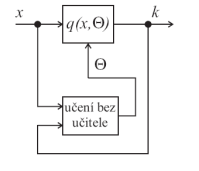
\includegraphics{image/bezu.png} 
\end{figure}

\subsection{Supervised learning}
Učení s učitelem, nebo supervised learning, je proces, kde model umělé inteligence je trénován na datové sadě, která obsahuje jak vstupní data, tak správné odpovědi (labely). Tento přístup umožňuje modelu naučit se předpovídat výstupy na základě nových vstupů na základě předchozích zkušeností. Tento typ učení je široce využíván v aplikacích jako je klasifikace (například rozpoznávání objektů na obrázcích) a regrese (například předpovídání cen nemovitostí), kde je důležité, aby model byl schopen správně identifikovat a reagovat na různé druhy dat.
\begin{figure}[h]
	\centering
	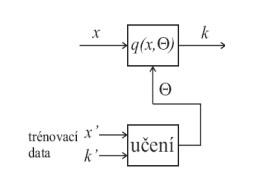
\includegraphics{image/su.png} 
\end{figure}


\subsection{Reinforcement learning}
Posilované učení, nebo reinforcement learning, je zase odlišné tím, že se zaměřuje na vývoj algoritmů, které se učí prostřednictvím interakce s prostředím a získávají zpětnou vazbu v podobě odměn nebo trestů. V tomto přístupu je agent, kterým může být například robot nebo software, vystaven prostředí, ve kterém se snaží provádět akce vedoucí k maximální možné odměně. Posilované učení je ideální pro situace, kde jsou rozhodnutí časově závislá a kde je třeba vzít v úvahu dlouhodobé důsledky akcí, jako jsou strategické hry, robotická navigace nebo autonomní řízení vozidel.
\begin{figure}[h]
	\centering
	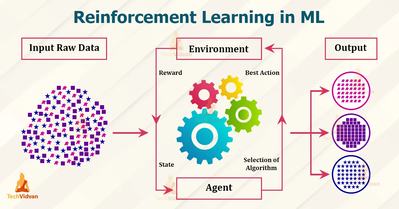
\includegraphics[width=0.8\linewidth, height=0.8\linewidth, keepaspectratio]{image/reinu.png}
	
\end{figure}

Pro maximalizaci celkové odměny je nezbytné, aby agent volil optimální akce v závislosti na svém současném stavu. Tento výběr akcí, známý jako strategie nebo politika $\pi$
, je klíčový pro přiřazení nejvhodnější akce pro každý stav. Existuje mnoho algoritmů pro určení efektivní funkce $\pi$
, nicméně zde se zaměříme specificky na Q-learning a jeho odvozené algoritmy.




\section{Q-learning}

Q-learning je algoritmus založený na principu posilovaného učení. Na rozdíl od metod, které přímo hledají optimální strategii $\pi$ (metody policy gradient), Q-learning postupuje nepřímo prostřednictvím tzv. Q-tabulky. Tato tabulka spojuje stavy s akcemi - každý řádek reprezentuje jeden stav a sloupce v tomto řádku různé akce. Agent vybírá akci s nejvyšší hodnotou v tabulce. Tyto hodnoty jsou známé jako Q-hodnoty, kde "Q" reprezentuje "quality" (kvalitu) akce. Algoritmus, který určuje nejlepší akci z Q-tabulky, je označován jako Q-funkce.
\begin{figure}[h]
	\centering
	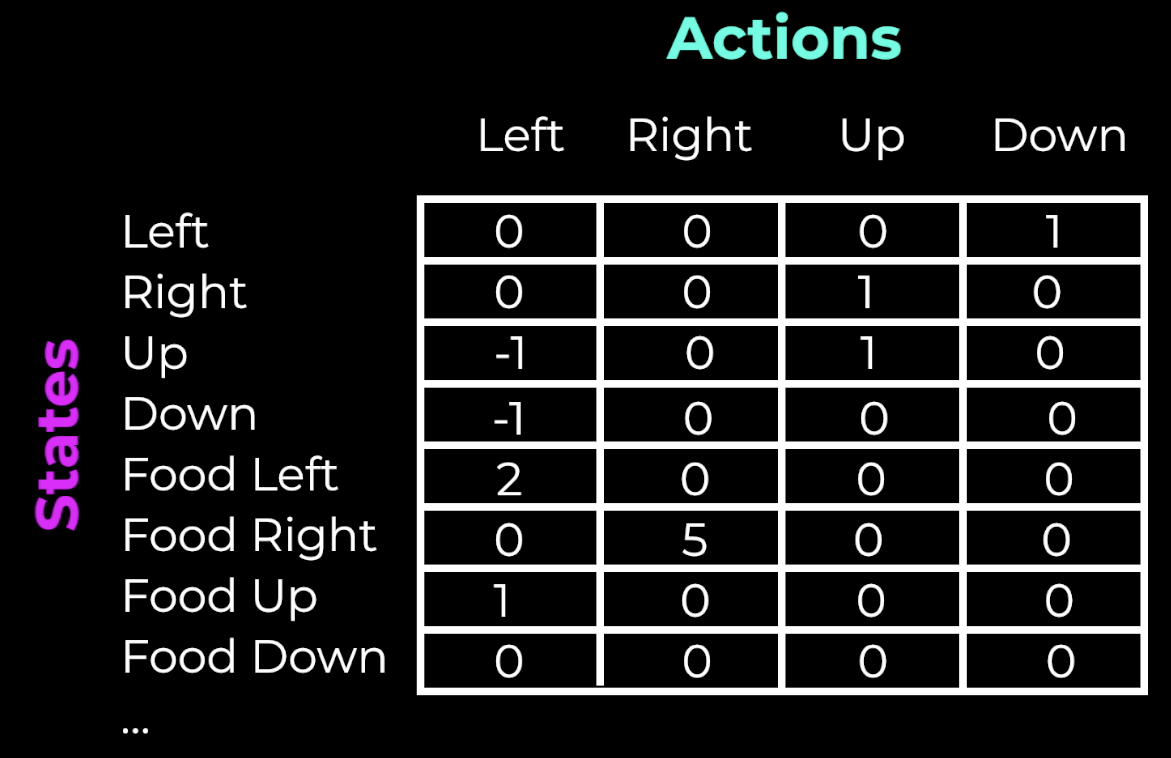
\includegraphics[width=0.8\linewidth, height=0.8\linewidth, keepaspectratio]{image/qlearn.png}
	
\end{figure}
Aktualizace Q-hodnot se provádí na základě odměn, které agent obdrží od prostředí za provedenou akci. Tato odměna, známá jako posílení, může být pozitivní, negativní (trest) nebo neutrální. Když agent obdrží za určitou akci negativní odměnu, dojde k snížení příslušné hodnoty v Q-tabulce, což vede k nižší pravděpodobnosti opětovného výběru této akce. Takto lze postupně eliminovat nežádoucí chování a podporovat chování, které je žádoucí.

\subsection{Okamžitá a dlouhodobá odměna}
Aktualizace Q-hodnot lze rozdělit na dvě zásadní části: okamžitou a dlouhodobou. Okamžitá část je reprezentována odměnou $r_{t}$, kterou agent obdrží za provedení akce $a_{t}$. K této okamžité odměně je pak přičítána dlouhodobá hodnota, reprezentující očekávané budoucí Q-hodnoty ze stavu $s_{t+1}$. Cílem je maximalizovat celkovou odměnu, zahrnující nejen aktuální, ale i budoucí akce. Například, v případě dvou možných akcí ($a_{1}$, $a_{2}$) ve stavu $s_{0}$ může být na první pohled akce s vyšší okamžitou odměnou méně výhodná v dlouhodobém horizontu, pokud by v důsledku jejího provedení následovaly stavy vedoucí k nižším celkovým odměnám.

\begin{figure}[h]
	\centering
	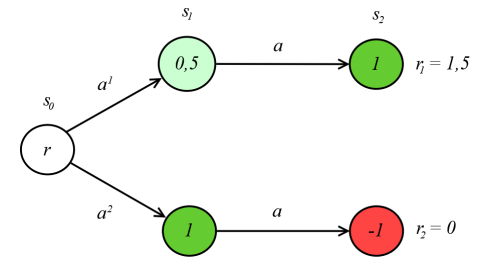
\includegraphics[width=0.8\linewidth, height=0.8\linewidth, keepaspectratio]{image/odmen.png}
\end{figure}[h]

Je klíčové najít správnou rovnováhu mezi okamžitou a dlouhodobou odměnou. Úloha dlouhodobé odměny může být upravena pomocí diskontního faktoru (discount factor) \(\gamma\), který určuje váhu budoucích odměn, zatímco míra učení (learning rate) \(\alpha\) ovlivňuje rychlost aktualizace Q-hodnot. Celkovou odměnu \(r\), skládající se z okamžité a dlouhodobé složky, lze vyjádřit jako součet těchto dvou komponent, s přihlédnutím k váze diskontního faktoru a míry učení.

\begin{equation}
	r=a.(r_{t}+\gamma . maxQ(s_{t+1,a}))
\end{equation}



V Q-tabulce se Q-hodnota pro daný stav a akci obvykle nepřepisuje přímo novou odměnou, ale upravuje se na základě již existující hodnoty. Toto se provádí za účelem zachování historických informací o výkonnosti dané akce. Aktualizační pravidlo pro Q-hodnoty tedy bude kombinovat aktuální odměnu s předešlými poznatky o daném stavu a akci, čímž se dosahuje efektivnějšího a přesnějšího učení.

\begin{equation}
	Q^{nova}(s_t,a_t)=(1-\alpha).Q(s_{t},a{t})+r
\end{equation}

\newpage
\subsection{Limitace Q-learningu}
Při použití Q-tabulky pro mapování stavů na akce v rámci Q-learningu se můžeme setkat s několika komplikacemi. Pro složitější úlohy, kde je stav určen několika proměnnými současně (například v 3D prostoru), může velikost Q-tabulky dosáhnout extrémních rozměrů, což vede k její nepraktičnosti. Navíc, protože stavy musí tvořit konečnou sadu, řešení spojitých stavů se stává problematickým. Další výzvou je manipulace s akcemi: v základním modelu Q-learningu jsou akce pouze přijaty nebo odmítnuty (binární výběr), což znemožňuje spojité řízení výstupu. Tyto problémy mohou být řešeny implementací umělých neuronových sítí, které nabízí flexibilnější a efektivnější přístup.



\newpage
\subsection{Deep Q-network}

Deep Q-network (DQN) je algoritmus, který byl vytvořen společností DeepMind v roce 2015. Tento algoritmus spojuje principy Q-learningu s umělou neuronovou sítí. Základním konceptem DQN je využití neuronové sítě, známé jako Q-síť, která nahrazuje tradiční Q-tabulku. Úkolem této sítě je co nejvíce přiblížit funkci Q-hodnoty. Vstupem do Q-sítě je stav $s_{t}$, a výstupem je reakce na tento stav $a_{t}$, což je podobné Q-tabulce. Nicméně, proces učení Q-sítě se liší od Q-tabulky, protože zde nelze jednoduše aktualizovat Q-hodnoty. Místo toho se Q-síť musí učit stejným způsobem jako jakákoliv jiná neuronová síť, a to využitím učení s učitelem, kde jsou všechny akce agenta stále hodnoceny pomocí odměňovací funkce a generují trénovací data.

Další rozdíl oproti klasickému Q-learningu je v aktualizačním pravidle. Vzhledem k tomu, že neuronovou síť neměníme přímo, vynecháváme část aktualizačního pravidla, která připočítává starou Q-hodnotu. Toto pravidlo aktualizace pak nabývá nové formy, která efektivně využívá schopnosti neuronové sítě k učení a přizpůsobení.

\begin{equation}
  Q^{nova}(s_t,a_t)=r_t+\gamma maxQ(s_{t+1},a)
\end{equation}


Neuronové sítě jsou efektivnější, když se učí na základě více dat, než jen jednoho výstupu. Efektivnějším přístupem je uchovávání historie předchozích stavů agenta. Zaznamenáváme stav, akci, odměnu a následující stav ($s_{t}$, $a_{t}$, $r_{t}$, $s_{t+1}$) - všechny elementy potřebné pro výpočet nových Q-hodnot. Během učení pak agent vybírá náhodně uspořádanou vzorku pevně stanovené velikosti z těchto uložených záznamů. Na základě této vzorky se počítají nové Q-hodnoty, které jsou poté uplatněny na neuronovou síť pomocí algoritmu zpětného šíření chyb. Tento proces uchovávání minulých stavů se nazývá metoda opakování zkušeností (experience replay).

\begin{figure}[h]
	\centering
	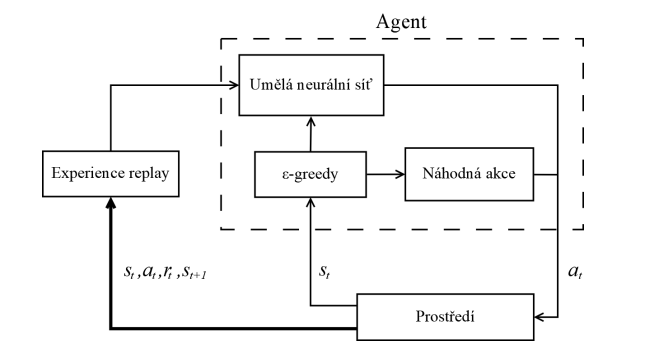
\includegraphics[width=0.8\linewidth, height=0.8\linewidth, keepaspectratio]{image/mod.png}
	
\end{figure}

\newpage
\section{Perceptron}
Perceptron v nejjednodušší podobě je binární klasifikátor, který mapuje vektory vstupů 
\(\mathbf{x} = [x_1, x_2, \ldots, x_n]\) na výstupní hodnoty \(f(\xi)\):
\[
f(\xi) = 
\begin{cases} 
	1 & \text{pro } \mathbf{w} \cdot \mathbf{x} - \theta \geq 0 \\
	0 & \text{jindy} 
\end{cases}
\]
kde \(\mathbf{w}\) je vektor vah a \(\theta\) je práh citlivosti neuronu.

Celkový podnět neuronu udává vážený součet \(\xi = \sum_{i=1}^{n} w_i \cdot x_i - \theta\). Tento celkový podnět bývá označován jako potenciál neuronu. Na potenciál reaguje neuron (perceptron) výstupní odezvou \(Z = f(\xi)\), kde \(f\) je tzv. přenosová funkce. Je-li přenosová funkce ve tvaru skokové funkce, perceptron funguje, jak již bylo řečeno, jako binární klasifikátor, neuron tedy dělí vstupní prostor na dvě části.
\begin{figure}[h]
	\centering
	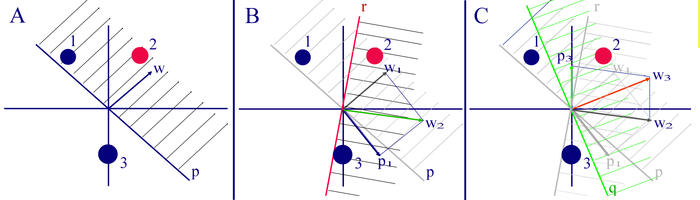
\includegraphics[width=0.8\linewidth, height=0.8\linewidth, keepaspectratio]{image/tri.png}
	
\end{figure}
Tři fáze učení jednoduchého perceptronu jsou následující:

\begin{enumerate}
	\item[A:] Je zvolen náhodně vektor vah \(\mathbf{w}\) a k němu určena kolmá rozhodovací hranice \(p\). Zjišťujeme výstup pro bod 1 - leží v oblasti s výstupem 1, i když má ležet v oblasti s výstupem 0. 
	\item[B:] Odečteme vektor bodu 1 od vektoru vah \(\mathbf{w_1}\) a získáme nový vektor vah \(\mathbf{w_2}\) a k němu příslušnou rozhodovací hranici znázorněnou přímkou \(r\). Bod 2 je umístěn správně, bodu 3 přiřadí síť hodnotu 1 i když má dostat výstup 0.
	\item[C:] Odečteme vektor bodu 3 od vektoru vah \(\mathbf{w_2}\) a získáme nový vektor vah \(\mathbf{w_3}\). Nyní je již problém vyřešen - všem bodům je přiřazen odpovídající hodnota výstupu. Řešením problému je tedy vektor vah \(\mathbf{w_3}\) s příslušnou rozhodovací hranicí \(q\).
\end{enumerate}



\newpage
\section{Multi layer perceptron(MLP)}

MLP je rozšířením dopředné neuronové sítě. Skládá se ze tří typů vrstev - vstupní vrstvy, výstupní vrstvy a skrytých vrstev. Vstupní vrstva přijímá vstupní signál k zpracování. Výstupní vrstva provádí požadované úlohy, jako jsou predikce a klasifikace. Libovolný počet skrytých vrstev, umístěných mezi vstupní a výstupní vrstvou, představuje skutečný výpočetní motor MLP. Podobně jako u dopředné sítě v MLP proudí data směrem dopředu od vstupní k výstupní vrstvě. Neurony v MLP jsou trénovány pomocí algoritmu učení zpětné propagace. MLP jsou navrženy tak, aby aproximovaly jakoukoli spojitou funkci a mohly řešit problémy, které nejsou lineárně separovatelné. Hlavními využitími MLP jsou klasifikace vzorů, rozpoznávání, predikce a aproximace.
\begin{figure}[h]
	\centering
	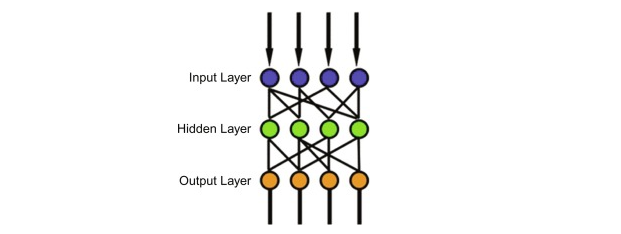
\includegraphics[width=0.8\linewidth, height=0.8\linewidth, keepaspectratio]{image/mul.png}
	
\end{figure}
\begin{equation}
	o_x = G(b_2 + W_2 h_x)
\end{equation}

\begin{equation}
	h_x = \Phi(x) = s(b_1 + W_1 x)
\end{equation}

s vektory zkreslení \( b_1, b_2 \); maticemi vah \( W_1, W_2 \) a aktivačními funkcemi \( G \) a \( s \). Sada parametrů k učení je sada \( \theta = \{W_1, b_1, W_2, b_2\} \). Typické volby pro \( s \) zahrnují tanh funkci s \( \text{tanh}(a) = \frac{e^a - e^{-a}}{e^a + e^{-a}} \) nebo logistickou sigmoidní funkci, s \( \text{sigmoid}(a) = \frac{1}{1 + e^{-a}} \).

\chapter{Využité postupy a technologie}
V průběhu projektu byly využity následující postupy a technologie:

\begin{itemize}
	\item \textbf{Umělé neuronové sítě:} Využití různých typů neuronových sítí pro modelování složitých vztahů a rozpoznávání vzorů.
	\item \textbf{Posilované učení:} Implementace algoritmů posilovaného učení, jako je Q-learning, pro efektivní rozhodování a adaptaci modelu.
	\item \textbf{Python a knihovny pro strojové učení:} Použití programovacího jazyka Python spolu s knihovnami jako PyTorch a Gym od OpenAI pro vývoj a trénování modelů.
	\item \textbf{Simulační prostředí:} Využití simulací pro testování a optimalizaci algoritmů umělé inteligence.
	\item \textbf{Data Analytics:} Analýza a zpracování dat pro lepší porozumění problému a efektivnější učení modelů.
\end{itemize}

\section{2D bludiště ovládané umělou inteligencí}

\subsection{Vytvoření a interakce s prostředím}
V rámci tohoto projektu je implementováno 2D bludiště, jehož navigaci řídí umělá inteligence. Pro vývoj a trénink AI modelu je využita knihovna PyTorch, což je oblíbený nástroj pro strojové učení napsaný v Pythonu, poskytující rozsáhlé možnosti pro práci s neurálními sítěmi. 

Pro simulaci interakce AI s bludištěm využíváme knihovnu Gym od OpenAI, která poskytuje standardizované rozhraní pro různé druhy simulovaných prostředí. Gym je rovněž napsána v Pythonu a je navržena tak, aby usnadňovala vývoj a testování algoritmů posilovaného učení.

\subsection{Ovládání bludiště}
Interakce mezi AI a bludištěm je realizována pomocí knihovny pynput. Tato knihovna umožňuje AI simulovat stisknutí kláves, čímž se umělá inteligence "naučí" ovládat bludiště. Pynput je psána v Pythonu a poskytuje jednoduchý způsob, jak generovat klávesové události, což je klíčové pro integraci AI s prostředím bludiště.

\subsection{Vykreslení prostředí}
Pro vykreslení bludiště byly použity dva různé herní enginy – Raylib a Pygame. Raylib je C knihovna, která se zaměřuje na snadné a rychlé vytváření aplikací a her, zatímco Pygame je sada Python modulů určených pro tvorbu her. Obě tyto knihovny byly vybrány pro jejich efektivitu a schopnost plynule vykreslovat grafické prvky bludiště, což je nezbytné pro realistickou simulaci a interakci AI s prostředím.





	
	\chapter*{Závěr}
	
	V rámci této práce jsme se zabývali využitím umělých neuronových sítí pro navigaci v bludišti, přičemž jsme se zaměřili na základní teoretické aspekty a praktickou aplikaci těchto technologií. Demonstrace AI modelu pro řešení bludišť zdůraznila potenciál neuronových sítí a současně odhalila výzvy spojené s jejich použitím.
	
	%% literatura
	\begin{thebibliography}{99}
		\bibitem{sablonaSOC} DOKULIL Jakub. \textit{Šablona pro psaní SOČ v programu \LaTeX} [Online]. Brno, 2020 [cit. 2020-08-24]. Dostupné z: \url{https://github.com/Kubiczek36/SOC_sablona}
		\bibitem{LaTeXprirucka}OETIKER, Tobias, Hubert PARTL, Irene HYNA, Elisabeth SCHEGL, Michal KOČER a Pavel SÝKORA. \textit{Ne příliš stručný úvod do systému LaTeX2e} [online]. 1998 [cit. 2020-08-24]. Dostupné z: \url{https://www.jaroska.cz/elearning/informatika/typografie/lshort2e-cz.pdf}
		\bibitem{wikibooksLaTeX}\textit{Wikibooks: LaTeX} [online]. San Francisco (CA): Wikimedia Foundation, 2001- [cit. 2020-08-24]. Dostupné z: \url{https://en.wikibooks.org/wiki/LaTeX}
		\bibitem{stackExchange} \textit{TeX - LaTeX Stack Exchange} [online]. Stack Exchange, 2020 [cit. 2020-09-01]. Dostupné z: \url{https://tex.stackexchange.com}
		\bibitem{sspuLogo} \textit{Střední škola průmyslová a umělecká Opava} [online]. [cit. 2023-11-11]. Dostupné z: \url{https://www.sspu-opava.cz}
		\bibitem{citacePRO}\textit{Citace PRO} [online]. Citace.com, 2020 [cit. 2020-08-31]. Dostupné z: \url{https://www.citacepro.com}
		\bibitem{Born2019} BORN, Max a Emil WOLF. \textit{Principles of optics: electromagnetic theory of propagation, interference and diffraction of light}. 7th (expanded) edition. Reprinted wirth corrections 2002. 15th printing 2019. Cambridge: Cambridge University Press, 2019. ISBN 978-0-521-64222-4.
	\end{thebibliography}
	
	%% obrázky 
	\listoffigures
	
	%% tabulky
	\listoftables
	
	\appendix %% začínají přílohy
	
	\titleformat{\chapter}[block]{\scshape\bfseries\LARGE}{Příloha \thechapter}{10pt}{\vspace{0pt}}[\vspace{-22pt}] %% nastavení nadpisu u příloh
	
	
	\chapter{%Příloha A 
		Spot diagramy a další }
	
	
\end{document}